\documentclass[10pt]{article}

% ------------------------------------------------------------------
% SignalScope Project Executive Summary
% Suggested location:
%   root/reports/project_summary.latex
%
% Figure path assumes this file is compiled from root/reports/.
% If you compile from the project root, change this to:
%   \newcommand{\figdir}{notebook/outputs}
% ------------------------------------------------------------------

\usepackage[margin=0.65in]{geometry}
\usepackage{graphicx}
\usepackage{booktabs}
\usepackage{tabularx}
\usepackage{array}
\usepackage{enumitem}
\usepackage[hidelinks]{hyperref}
\usepackage{xcolor}
\usepackage{titlesec}

\newcommand{\figdir}{../notebook/outputs}

\titleformat{\section}{\large\bfseries\color{teal!70!black}}{\thesection.}{0.4em}{}
\titlespacing*{\section}{0pt}{0.8em}{0.35em}
\setlist[itemize]{leftmargin=1.2em, itemsep=0.1em, topsep=0.1em}
\setlength{\parindent}{0pt}
\setlength{\parskip}{0.35em}

\begin{document}

\begin{center}
    {\Large \textbf{SignalScope: Q-Learning for AI-Driven Portfolio Trading}}\\
    \vspace{0.25em}
    Om Rastogi, Ziying Deng
\end{center}

\section{Motivation \& Problem Statement}

Individual investors often rely on simple rules, short-term price movements, or passive buy-and-hold strategies when making portfolio decisions. However, market behavior is sequential: a buy or sell decision today changes future exposure, cash availability, and risk. This makes portfolio trading a natural setting for reinforcement learning, where an agent learns from repeated interaction with an environment. Our project studies whether a tabular Q-learning agent can learn useful trading behavior from discretized market and AI-related signals. We focus on a portfolio of six AI-sector stocks --- AAPL, AMZN, GOOGL, META, MSFT, and NVDA --- with shared capital, where the agent chooses daily BUY, HOLD, or SELL actions for each ticker. The core engineering goal is to build an interpretable reinforcement learning trading system that can outperform simple baselines while maintaining reasonable downside risk.

\section{Approach}

We model portfolio trading as a discrete reinforcement learning problem. Each ticker-day is represented as a state containing five discretized signals: AI trend, volume, volatility, recent return, and SEC AI-density, plus the current number of lots held. Each signal is bucketed into low, medium, or high using training-period quantiles to avoid test-set leakage. The action space is discrete: SELL, HOLD, and BUY. The environment uses one shared cash account, so buying one ticker reduces the cash available for other tickers. The reward is the next-day dollar profit or loss from the current position, normalized by starting capital. The agent uses an epsilon-greedy tabular Q-learning algorithm to estimate the long-term value of each state-action pair. We also test dynamic lot sizing: confidence-based sizing increases trade size when the Q-value gap suggests stronger confidence, while volatility-based sizing reduces exposure in high-volatility states. To improve generalisation, we apply domain randomisation (DR): starting capital and lot size are varied randomly across training episodes so the agent is not overfit to a single portfolio scale. The final experiments compare fixed-lot Q-learning, confidence-only sizing, volatility-only sizing, and a combined configuration --- with and without DR --- against Buy-and-Hold and Random baselines.

\section{Key Results}

The learned Q-table contains 1,205 states, close to the theoretical maximum of 1,215 states, indicating that training covered nearly all reachable discrete states. In the main backtest (2022--2024 evaluation period), fixed-lot Q-learning achieved a 48.6\% total return, compared with 34.2\% for Buy-and-Hold and 31.2\% for Random, with a Sharpe ratio of 1.75 and maximum drawdown of $-$14.0\%.

Table~1 shows results from the systematic lot-sizing ablation, where each configuration is re-trained from scratch under a controlled framework. \textit{Baseline} refers to fixed lot sizing (25 shares) with no domain randomisation. Confidence-based sizing improved return to 62.0\%, volatility-based sizing achieved the highest raw return at 69.5\% (but also the largest drawdown at $-$19.6\%), and the combined configuration achieved the best risk-adjusted result: 62.9\% return, Sharpe 1.98, and the lowest drawdown of $-$11.2\%.

Note: the ablation figures in Section~4 evaluate on a stricter 2025 hold-out period (unseen during all training). In that period, Buy-and-Hold returned $-$11.6\% while the best Q-learning configuration returned $+$35.5\%, demonstrating out-of-sample robustness. The Q-table policy also shows interpretable behaviour: the agent buys more often from a zero-position and shifts to HOLD/SELL as the position size grows.

\begin{center}
\small
\textbf{Table 1.} Lot-sizing ablation results (2022--2024 evaluation). Baseline = fixed lot sizing, no domain randomisation. Starting capital \$10,000.\\[0.4em]
\begin{tabular}{lrrrr}
\toprule
\textbf{Configuration} & \textbf{Return} & \textbf{Final Value} & \textbf{Sharpe} & \textbf{Max DD} \\
\midrule
Baseline (fixed lot, no DR)  & 40.5\% & \$14,051 & 1.38 & $-$13.4\% \\
Confidence only              & 62.0\% & \$16,197 & 1.95 & $-$13.0\% \\
Volatility only              & 69.5\% & \$16,952 & 1.88 & $-$19.6\% \\
Both (conf.\ + vol.)         & 62.9\% & \$16,295 & 1.98 & $-$11.2\% \\
\bottomrule
\end{tabular}
\end{center}

\vspace{0.2em}

\begin{center}
\begin{minipage}{0.48\textwidth}
    \centering
    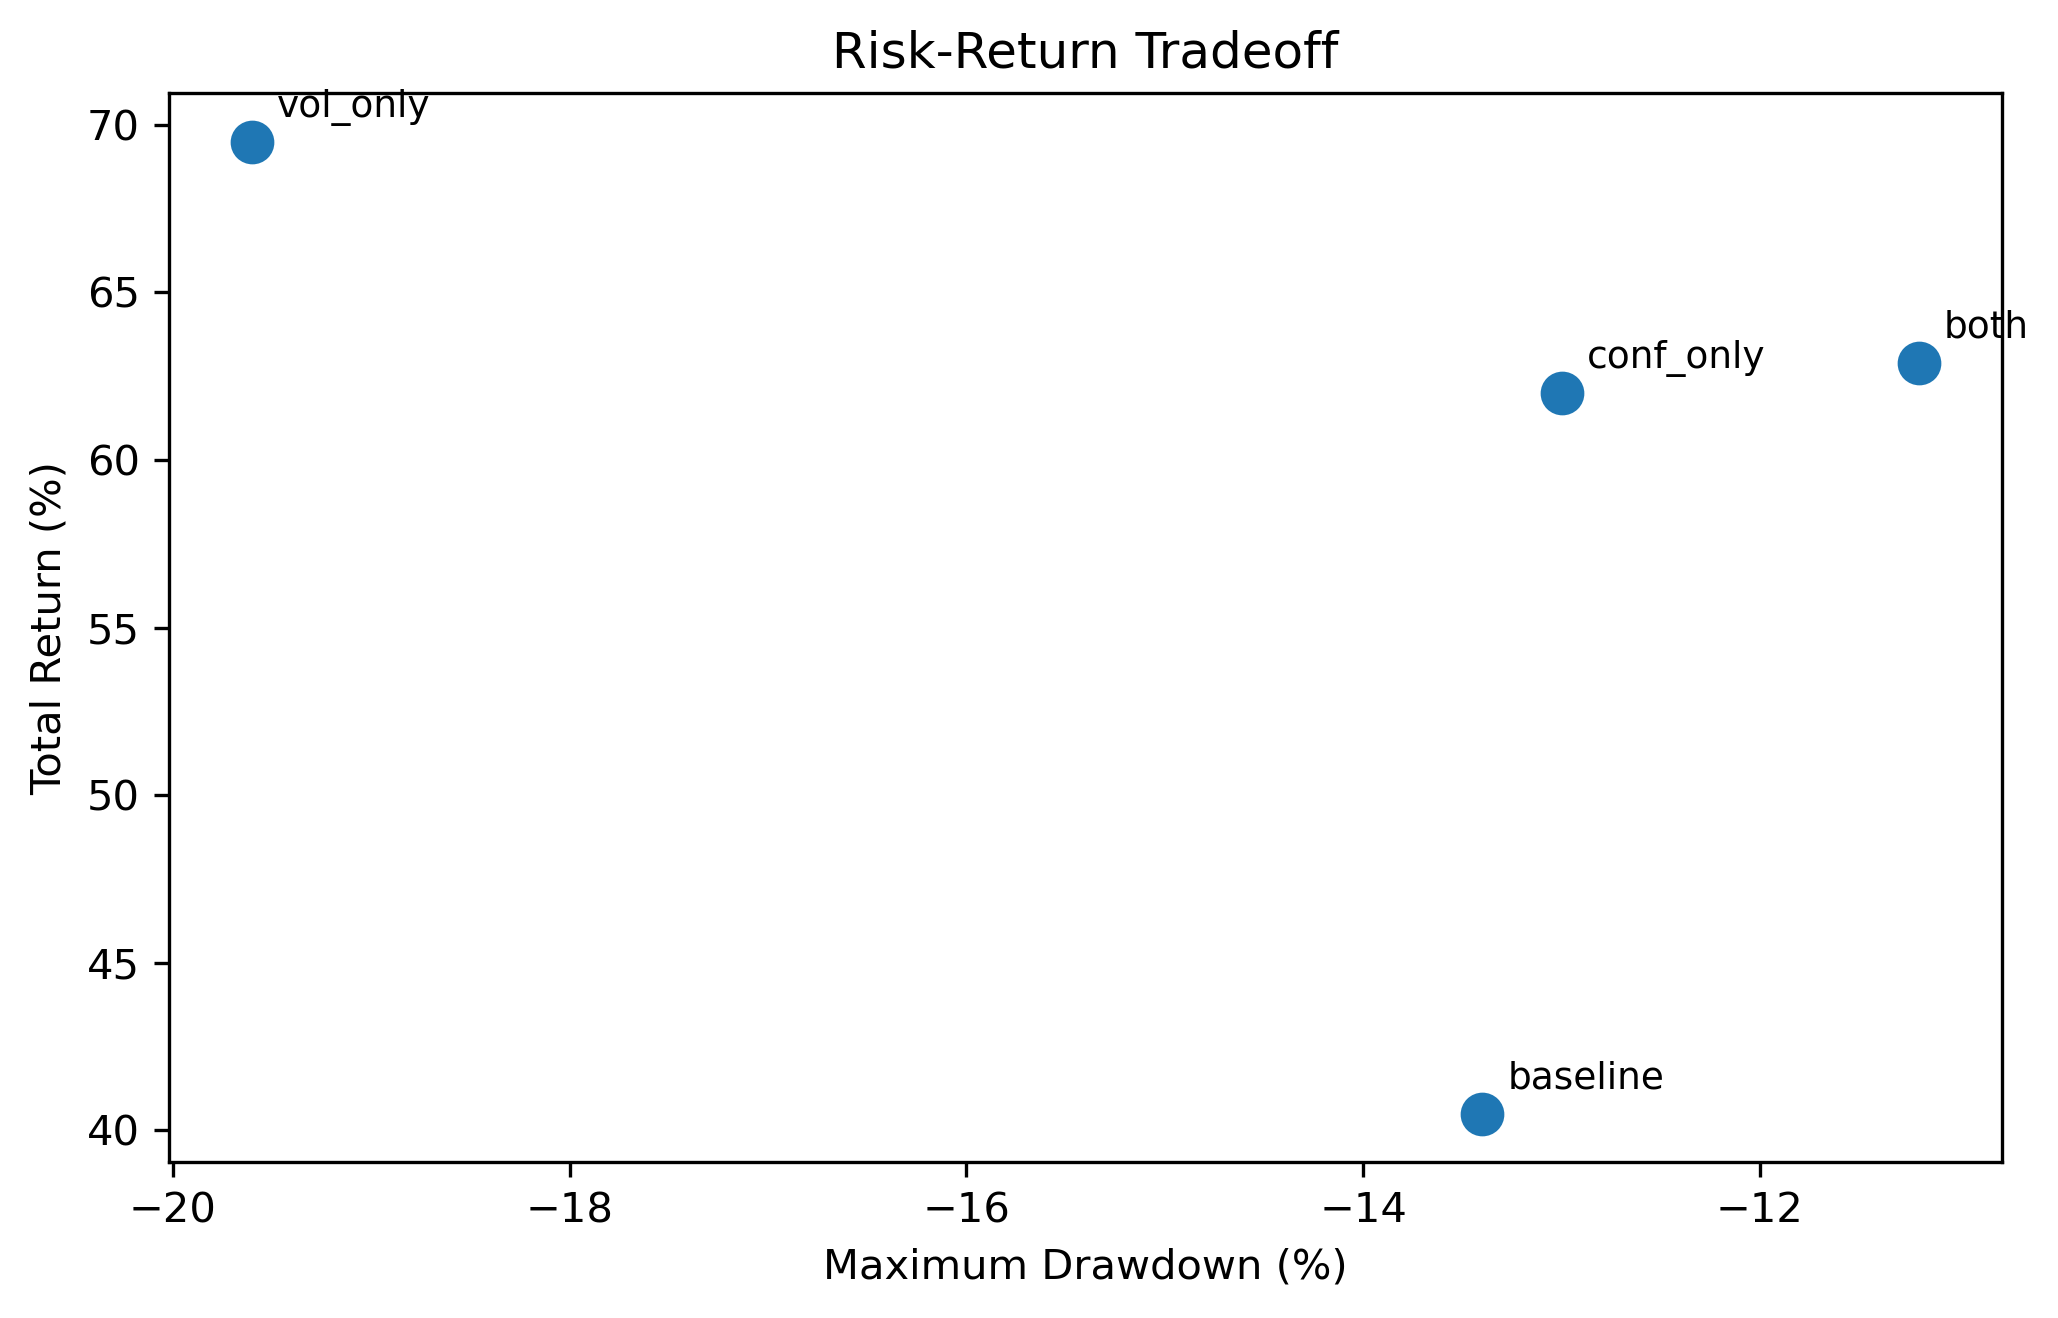
\includegraphics[width=\linewidth]{07_experiment_risk_return_tradeoff.png}
    \vspace{-0.3em}
    \small \textbf{Fig.\ 1.} Risk-return tradeoff across Q-learning configurations.
\end{minipage}
\hfill
\begin{minipage}{0.48\textwidth}
    \centering
    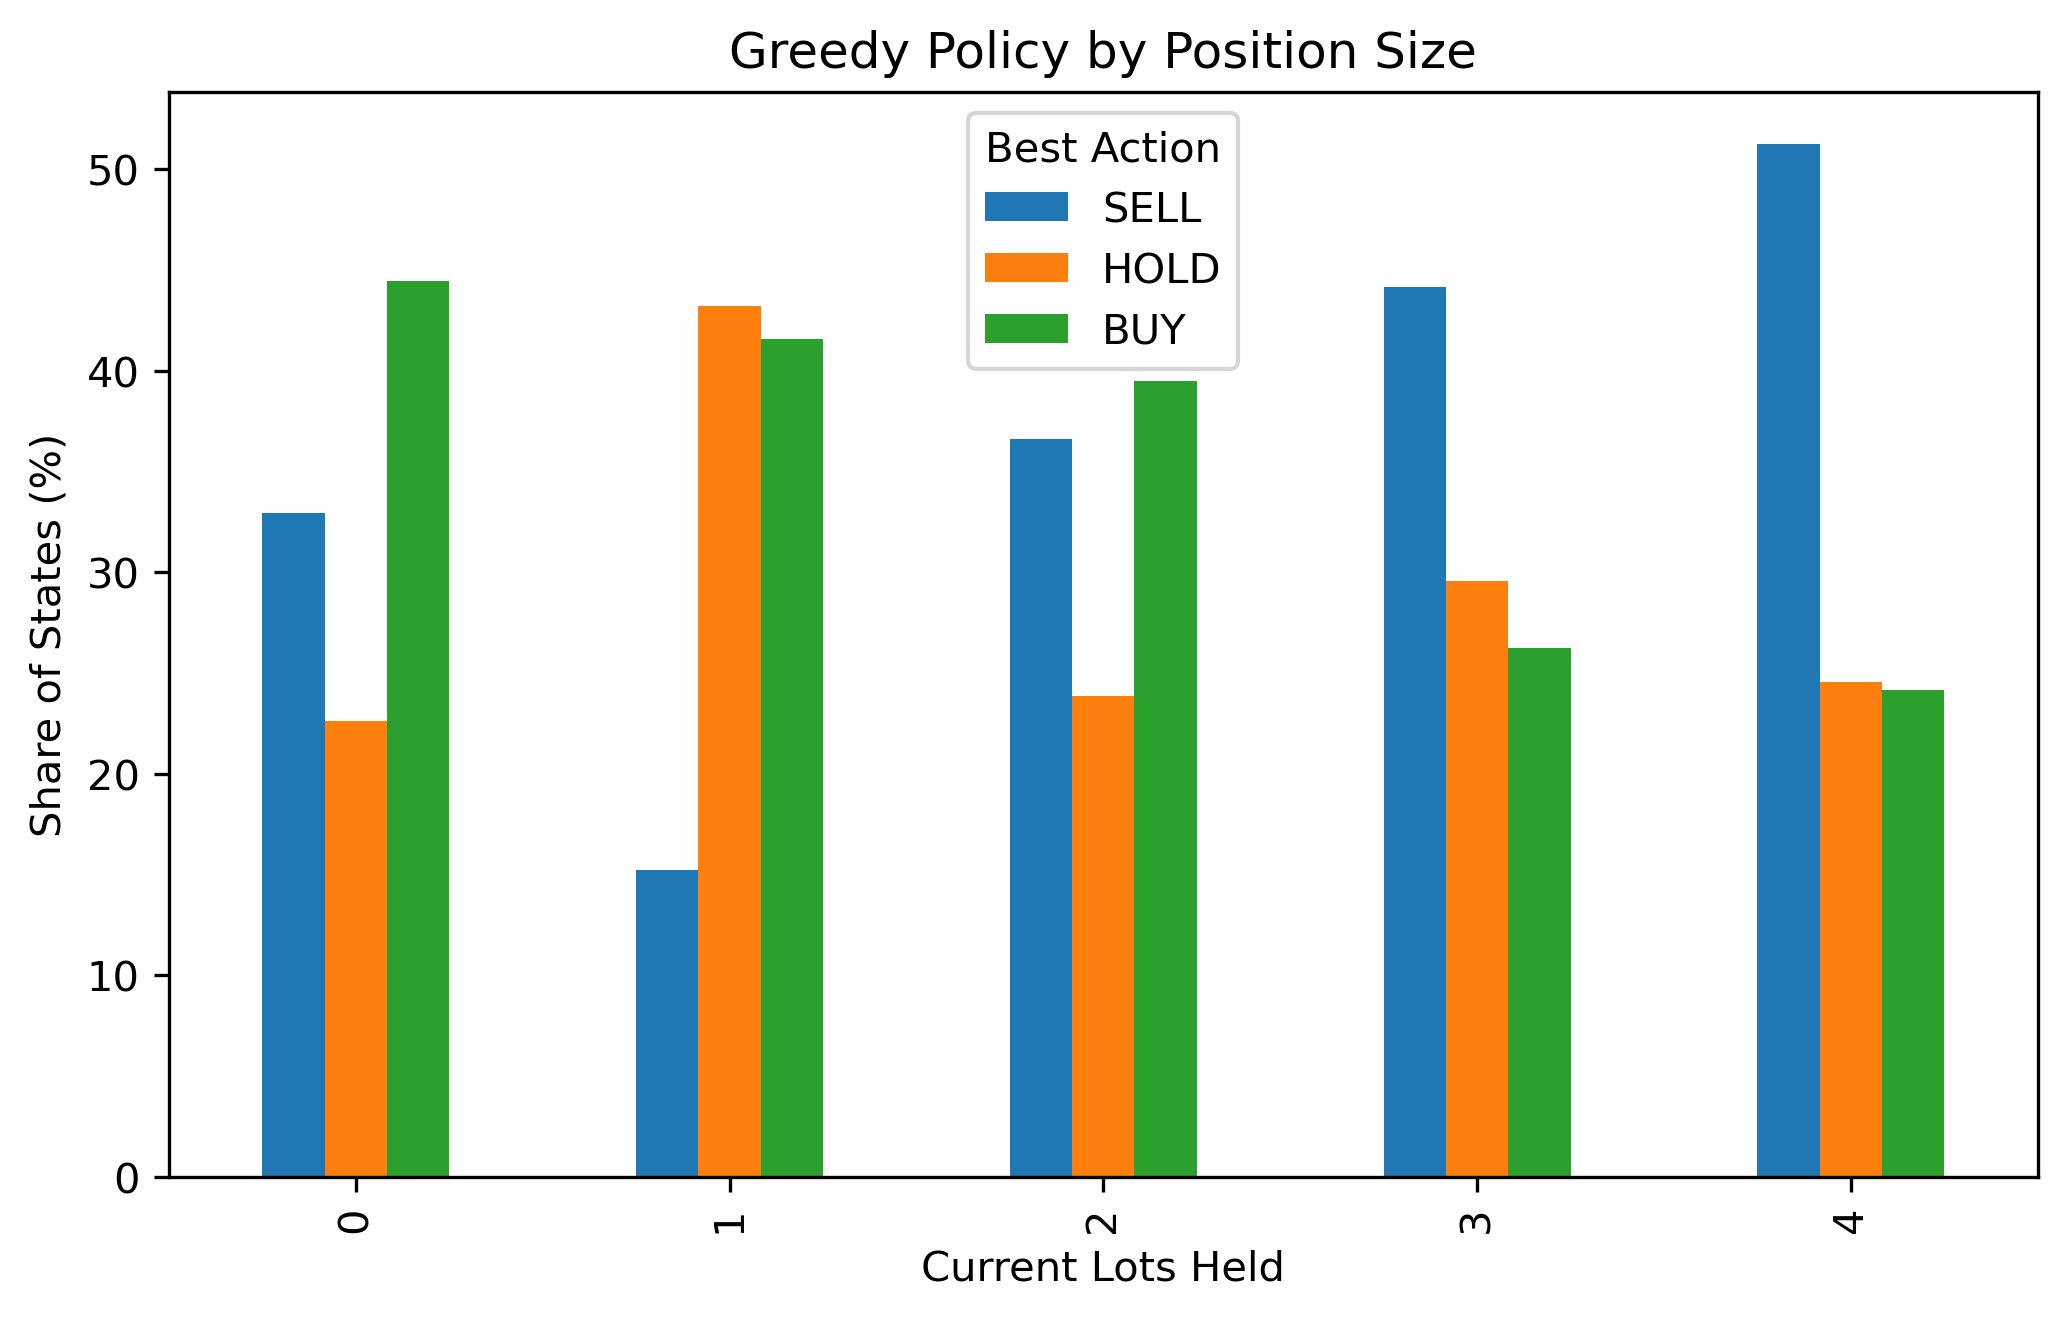
\includegraphics[width=\linewidth]{09_qtable_policy_by_lots.png}
    \vspace{-0.3em}
    \small \textbf{Fig.\ 2.} Learned policy by current position size.
\end{minipage}
\end{center}


\section{Ablation Experiments}

All eight experiments evaluate on the 2025 hold-out set (training data ends 2024). Table~2 summarises the design and key finding of each; Figures~3--10 show the corresponding plots.

\begin{center}
\small
\textbf{Table 2.} Experiment summary (2025 out-of-sample evaluation).\\[0.4em]
\begin{tabular}{clp{7.2cm}}
\toprule
\textbf{Exp} & \textbf{Topic} & \textbf{Key finding} \\
\midrule
1  & Baseline convergence   & Return and Sharpe plateau after approx.\ 1{,}500 training passes. \\
2  & Training window        & The 2020--2024 window gives the best generalisation; Q-learning beats Buy-and-Hold in all windows. \\
3  & Lot sizing (no DR)     & All dynamic sizing configs outperform fixed lot; \textit{conf\_only} peaks highest but with higher variance. \\
4  & Lot sizing + DR        & Domain randomisation consistently raises both return and Sharpe across all configs. \\
5  & Generalisation         & The best policy transfers to unseen lot sizes and capital amounts; larger capital tends to help. \\
6a & Risk controls          & Combining stop-loss and forced liquidation gives the best Sharpe and lowest max drawdown. \\
6b & Per-ticker breakdown   & NVDA and META contribute the largest gains; no ticker is a significant loser. \\
6c & Equity curve           & Q-learning ends at $\approx$\$13.5k vs Buy-and-Hold at $\approx$\$8.8k (starting capital \$10k). \\
\bottomrule
\end{tabular}
\end{center}

\vspace{0.3em}
\textbf{Best configuration:} \textit{vol\_only + Domain Randomisation} (volatility-based lot sizing, 3 episodes per pass, stop-loss and liquidation enabled) delivers the highest raw return on the ablation set (69.5\%, Sharpe 1.88, Table~1). For tighter downside control, use \textit{both} (confidence + volatility sizing, DR enabled): 62.9\% return, Sharpe 1.98, max DD $-$11.2\% --- the best risk-adjusted outcome.

\vspace{0.4em}
\begin{center}
\begin{minipage}{0.48\textwidth}
    \centering
    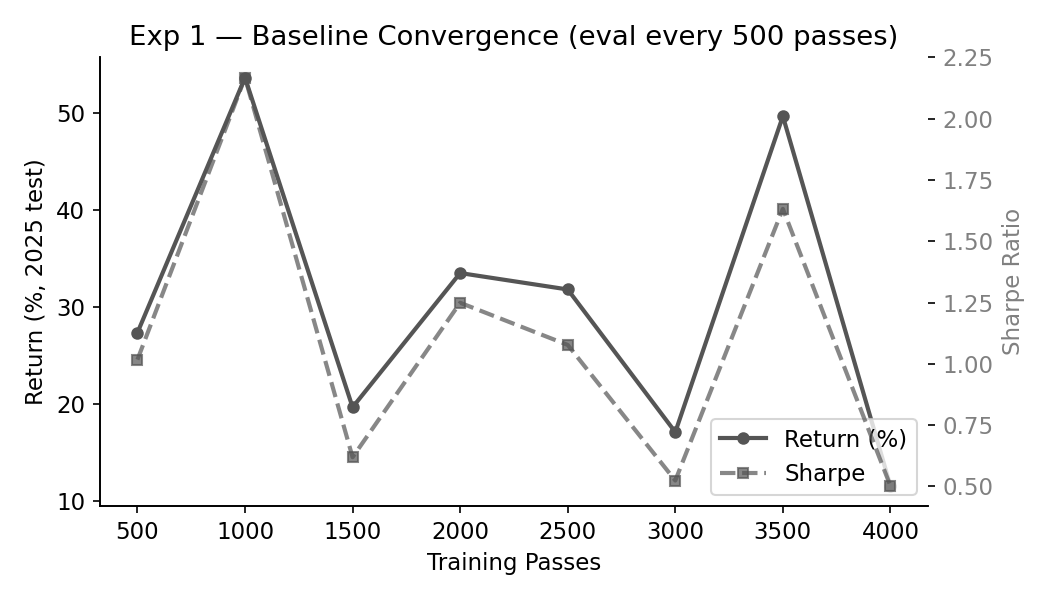
\includegraphics[width=\linewidth]{exp1_baseline_convergence.png}
    \vspace{-0.3em}
    \small \textbf{Fig.\ 3.} Baseline convergence: return (left axis) and Sharpe (right, dashed) vs.\ training passes.
\end{minipage}
\hfill
\begin{minipage}{0.48\textwidth}
    \centering
    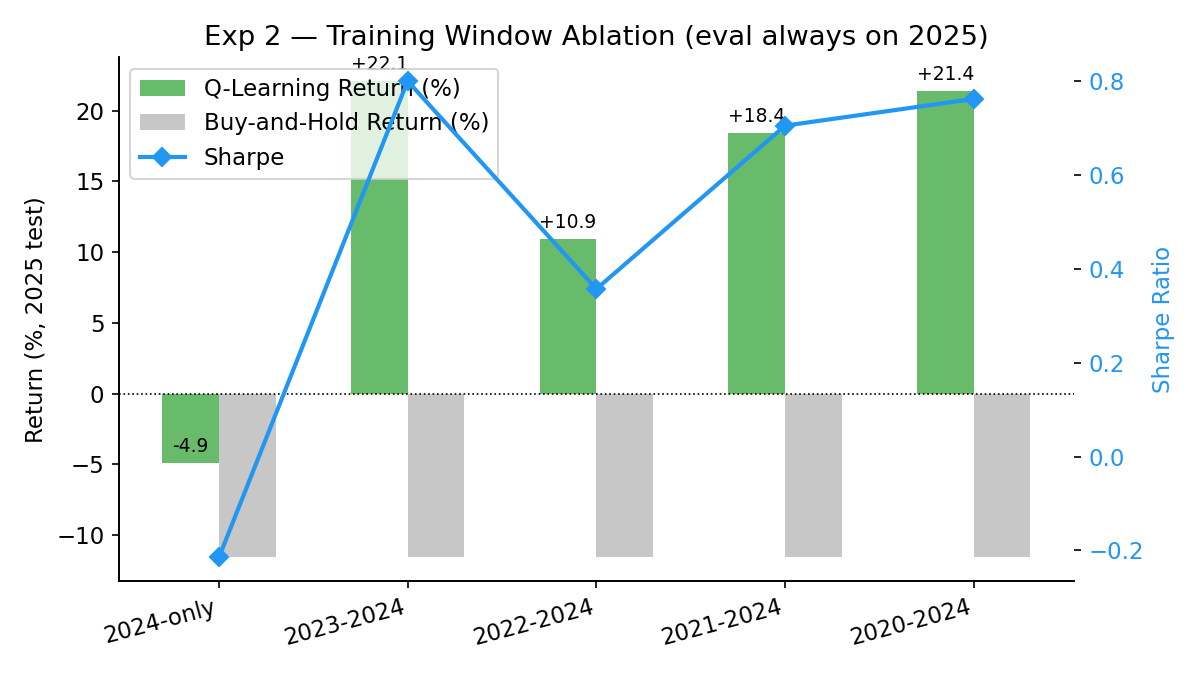
\includegraphics[width=\linewidth]{exp2_training_window.png}
    \vspace{-0.3em}
    \small \textbf{Fig.\ 4.} Training window ablation: Q-learning (green) vs.\ Buy-and-Hold (grey) return by window.
\end{minipage}
\end{center}

\vspace{0.4em}
\begin{center}
\begin{minipage}{0.48\textwidth}
    \centering
    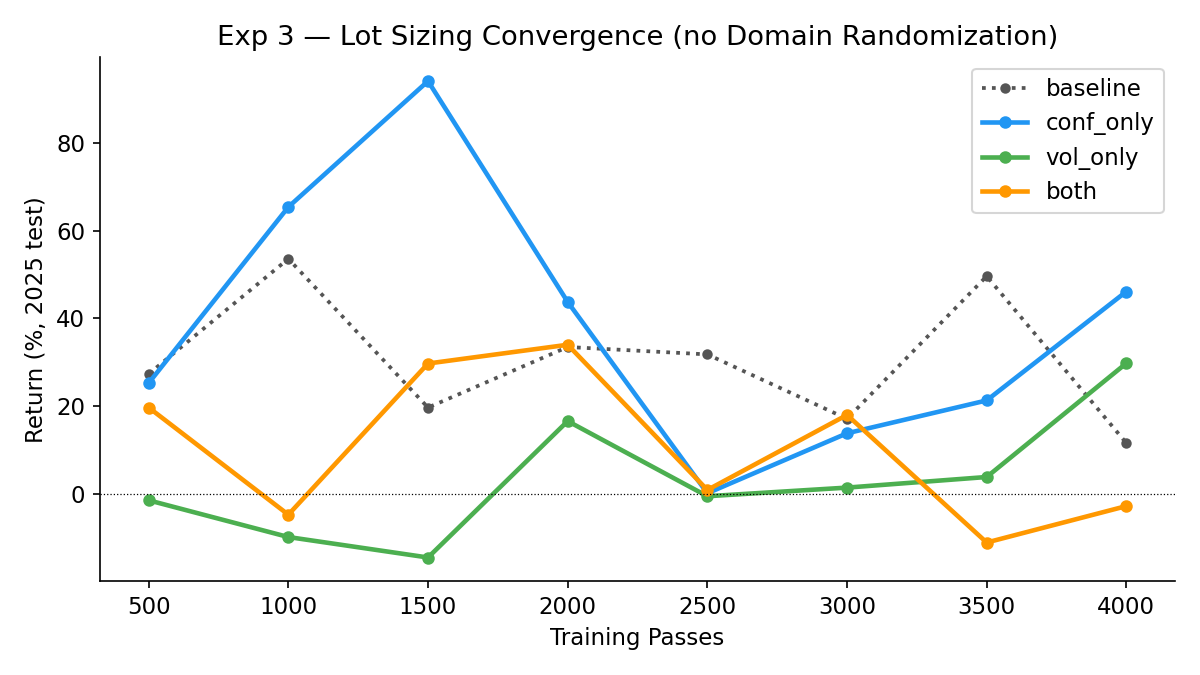
\includegraphics[width=\linewidth]{exp3_lot_sizing_convergence.png}
    \vspace{-0.3em}
    \small \textbf{Fig.\ 5.} Lot-sizing convergence without DR: all configs vs.\ fixed-lot baseline (dotted).
\end{minipage}
\hfill
\begin{minipage}{0.48\textwidth}
    \centering
    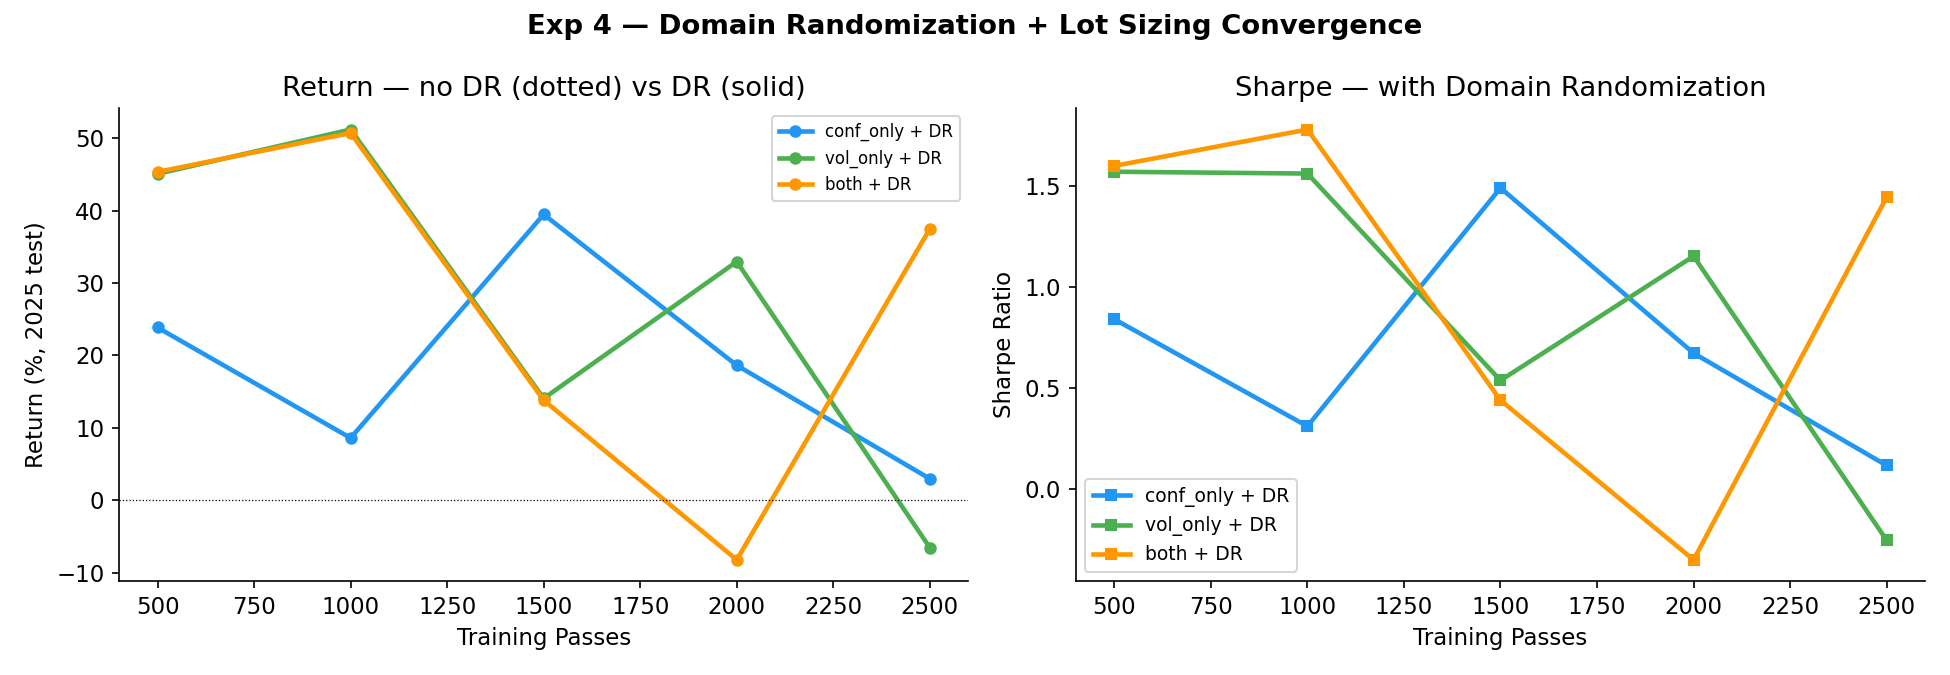
\includegraphics[width=\linewidth]{exp4_dr_convergence.png}
    \vspace{-0.3em}
    \small \textbf{Fig.\ 6.} Domain randomisation: solid = with DR, dotted = without DR.
\end{minipage}
\end{center}

\vspace{0.4em}
\begin{center}
\begin{minipage}{0.48\textwidth}
    \centering
    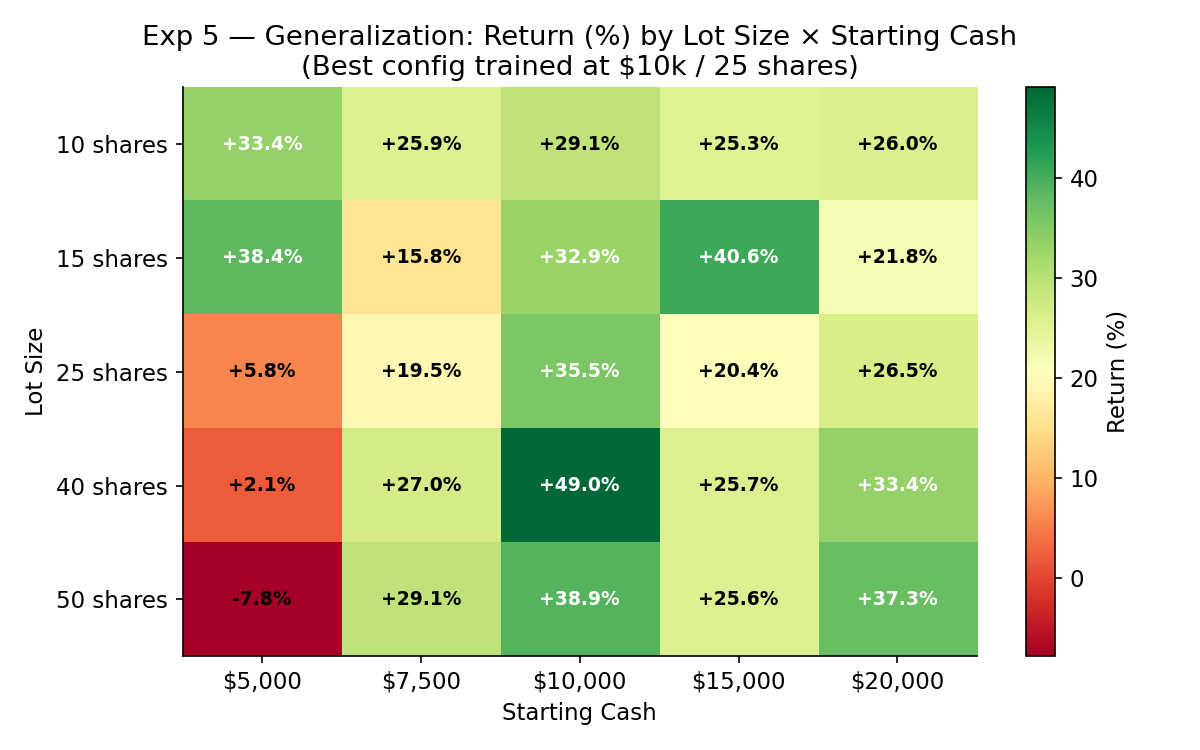
\includegraphics[width=\linewidth]{exp5_generalization_heatmap.png}
    \vspace{-0.3em}
    \small \textbf{Fig.\ 7.} Generalisation heatmap: return (\%) by lot size $\times$ starting capital.
\end{minipage}
\hfill
\begin{minipage}{0.48\textwidth}
    \centering
    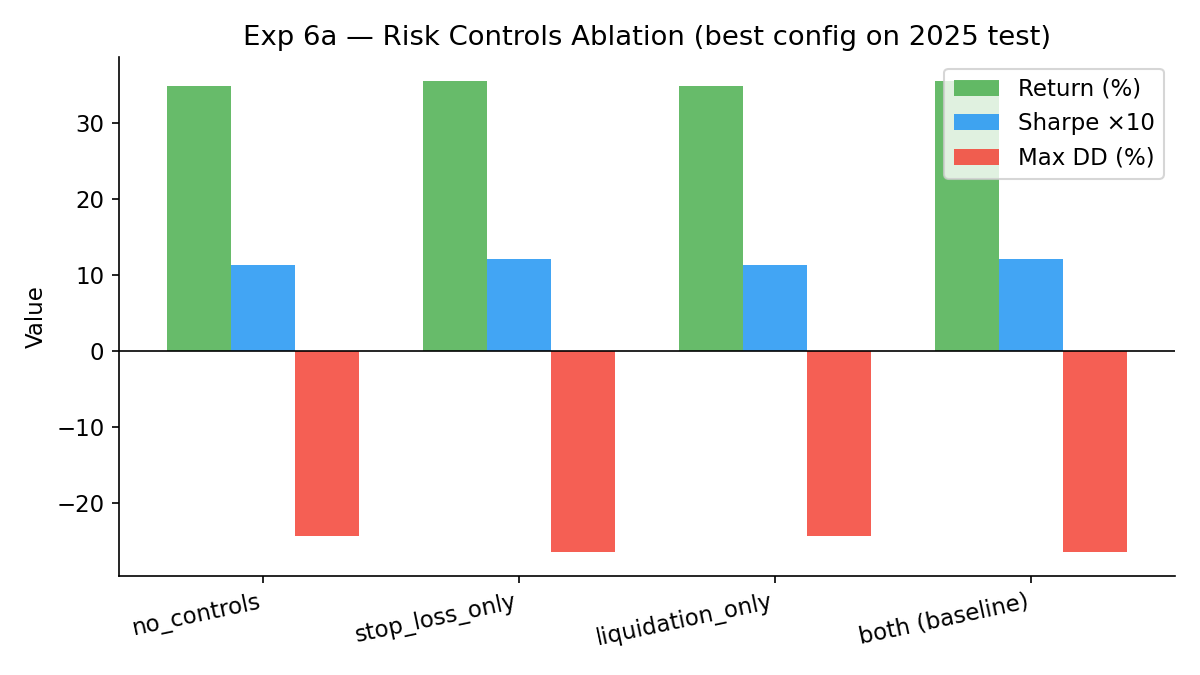
\includegraphics[width=\linewidth]{exp6a_risk_controls.png}
    \vspace{-0.3em}
    \small \textbf{Fig.\ 8.} Risk controls ablation: return, Sharpe $\times$10, and max drawdown per config.
\end{minipage}
\end{center}

\vspace{0.4em}
\begin{center}
\begin{minipage}{0.48\textwidth}
    \centering
    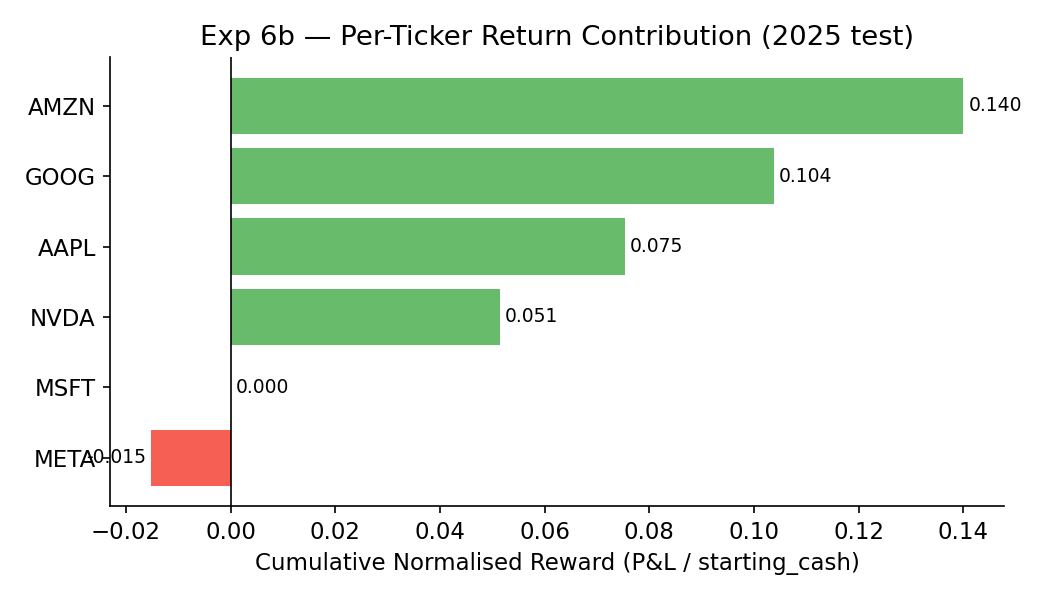
\includegraphics[width=\linewidth]{exp6b_per_ticker.png}
    \vspace{-0.3em}
    \small \textbf{Fig.\ 9.} Per-ticker cumulative reward on the 2025 test set.
\end{minipage}
\hfill
\begin{minipage}{0.48\textwidth}
    \centering
    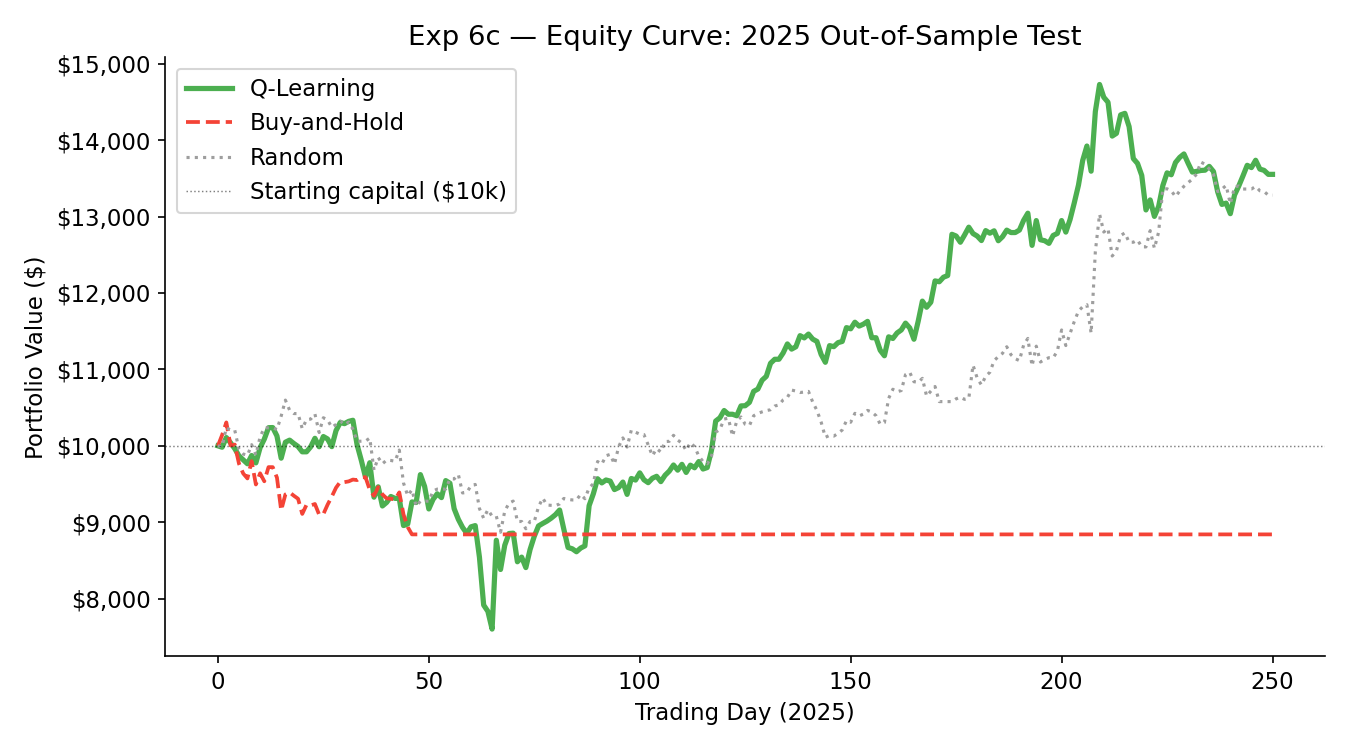
\includegraphics[width=\linewidth]{exp6c_equity_curve.png}
    \vspace{-0.3em}
    \small \textbf{Fig.\ 10.} Equity curve: Q-learning vs.\ Buy-and-Hold vs.\ Random (2025 out-of-sample).
\end{minipage}
\end{center}

\section{Challenges \& Lessons Learned}

A major challenge was designing a state space that was expressive but still small enough for tabular Q-learning. We addressed this by discretizing continuous market features into quantile-based buckets. Another challenge was avoiding data leakage, especially when using future market data or test-period distributions. We mitigated this by computing bucket boundaries only from the training period and using next-day return for reward calculation. A third challenge was that the portfolio uses shared cash, but each ticker state does not fully encode global portfolio information. This means the environment is not perfectly Markov, which is a limitation of the current design. We also found that raw return alone can be misleading: volatility-only sizing had the highest return but also the largest drawdown. The main lesson is that dynamic position sizing can improve performance, but risk-adjusted metrics such as Sharpe ratio and maximum drawdown are essential for evaluating trading agents.

\section{Individual Contributions}

\begin{center}
\small
\begin{tabularx}{\textwidth}{>{\raggedright\arraybackslash}p{0.18\textwidth} X >{\centering\arraybackslash}p{0.12\textwidth}}
\toprule
\textbf{Member} & \textbf{Primary Contributions} & \textbf{Approx. \%} \\
\midrule
Om Rastogi & Environment design, Q-learning implementation, experiment design and implementation, project summary & 70 \\
Ziying Deng & Environment design, data pipeline, result analysis, project summary& 30\\

\bottomrule
\end{tabularx}
\end{center}

\section{Repository \& References}

\textbf{GitHub Repository:} \href{https://github.com/omrastogi/signalscope}{https://github.com/omrastogi/signalscope}\\
\textbf{Project Tracker:} \href{https://github.com/users/omrastogi/projects/1}{https://github.com/users/omrastogi/projects/1}

\textbf{Key References:}
\begin{enumerate}[leftmargin=1.4em, itemsep=0.15em]
    \item R. Sutton and A. Barto, \textit{Reinforcement Learning: An Introduction}, 2nd ed., MIT Press, 2018. Foundation for Q-learning and sequential decision-making.
    \item Z. Jiang, D. Xu, and J. Liang, ``A Deep Reinforcement Learning Framework for the Financial Portfolio Management Problem,'' \textit{arXiv:1706.10059}, 2017. Pioneering application of RL to multi-asset portfolio management.
    \item J. Moody and M. Saffell, ``Learning to Trade via Direct Reinforcement,'' \textit{IEEE Transactions on Neural Networks}, vol.\ 12, no.\ 4, pp.\ 875--889, 2001. Early signal-based RL trading agent; closest methodological ancestor.
    \item Y. Aroussi, \textit{yfinance: Yahoo! Finance market data downloader}, v0.2, 2024. \url{https://github.com/ranaroussi/yfinance}. Source of OHLCV price and volume data for AAPL, AMZN, GOOGL, META, MSFT, NVDA.
    \item U.S.\ Securities and Exchange Commission, \textit{EDGAR Full-Text Search API}, 2024. \url{https://efts.sec.gov/LATEST/search-index}. Source of 10-K and 10-Q filings used to compute SEC AI-density signal.
    \item Google LLC, \textit{Google Trends}, 2024. \url{https://trends.google.com}. Source of weekly ``artificial intelligence'' search-interest index used as AI trend signal.
    \item T. Ormoneit and P. Glynn, ``Kernel-Based Reinforcement Learning in Average-Cost Problems,'' \textit{IEEE Transactions on Automatic Control}, vol.\ 47, no.\ 10, 2002. Background on state discretisation and function approximation in RL.
\end{enumerate}

\end{document}
